\begin{fex}
Soit $f$ l'application définie par:
\[
f \colon z \mapsto \frac{\exp(iaz)}{1+z^2}
\]
avec $a>0$ réel. 
\begin{enumerate}
  \item En utilisant la première formule de Cauchy, évaluer l'intégrale de $f$
  le long du contour donné figure \ref{fig:contour_ex1} et sous l'hypothèse
  $R>1$.
  \item Par passage à la limite $R \to +\infty$, en déduire la transformée de
  Fourier de l'application $x \mapsto (1+x^2)^{-1}$.
\end{enumerate}
\end{fex}
\begin{figure}[ht]
\includegraphics[scale=0.3]{contour_ex1.pdf}
\caption{Contour d'intégration}\label{fig:contour_ex1}
\end{figure}
\begin{enumerate}
 \item Pour $R > 1$, le point $i$ se trouve à l'intérieur du contour
d'intégration $\gamma$. On a donc:
\[
 \int_\gamma \frac{\exp(iaz)}{z+i} \frac{dz}{z-i} = i 2 \pi \frac{\exp(-a)}{2i}
= \pi \exp(-a)
\]
\item On applique le lemme de Jordan:
\[
\left|z\frac{\exp(iaz)}{z^2+1}\right| = \frac{|z|\exp(-a\Im(z))}{|1+z^2|}
\]
Sur le demi-cercle, $\Im(z) \leq 0$, d'où:
\[
\frac{|z|\exp(-a\Im(z))}{|1+z^2|} \leq \frac{R}{R^2-1}
\]
qui a pour limite 0 lorsque $R \to +\infty$.
\item On obtient immédiatement que pour $\xi > 0$, la transformée de Fourier a
pour valeur $\pi \exp(-\xi)$. Par parité, elle vaut donc sur tout $\R$,
$\pi \exp(-|\xi|)$.

\end{enumerate}

%\begin{figure}[ht]
%\includegraphics[scale=0.3]{images/contour_ex1.pdf}
%\caption{Contour d'intégration}\label{fig:contour_ex1}
%\end{figure}
\begin{fex}
    En utilisant la première formule de Cauchy, calculer la valeur de l'intégrale:
    \[
    \int_0^{2\pi} \frac{1}{2 + \sin x} dx
    \]
    \leftline{\textbf{Indication:}}
    Écrire le sinus sous la forme:
    \[
\sin x =\frac{e^{ix}-e^{-ix}}{2i}
    \]
    et vérifier que l'intégrale précédente est une intégrale d'une fraction rationnelle sur un lacet dans le plan
    complexe.
\end{fex} 
Quand $x$ parcourt $[0;2\pi]$ et en remplaçant $\sin$ par $e^{ix}$, on va chercher à écrire l'intégrale comme une fraction en $e^{ix}$ et intégrer sur le cercle unité. 
\begin{align*} 
    \int_0^{2\pi} \frac{1}{2 + \sin x} dx 
    &= \int_0^{2\pi} \frac{1}{2 + \frac{e^{ix}-e^{-ix}}{2i}} dx \\ 
    &= \int_0^{2\pi} \frac{2ie^{ix}}{4ie^{ix} + e^{2ix}-1} dx \\  
    &= \int_{C(0,1)} \frac{2}{4iz + z^2 - 1} dz 
\end{align*} 
Le dénominateur admet pour racines $z_1 = (-2-\sqrt{3})i$ (à l'extérieur du cercle unité) et $z_2 = (-2+\sqrt{3})i$ (à l'intérieur du cercle). 

Une application de la première formule de Cauchy donne 
\begin{align*} 
    \int_0^{2\pi} \frac{1}{2 + \sin x} dx 
    &= 2i \pi I(C(0,1), z_2) \frac{2}{z_2-z_1} \\ 
    &= \frac{2\pi}{\sqrt{3}} 
\end{align*} 